\documentclass[conference]{IEEEtran}
\ifCLASSINFOpdf

\else

\fi
\usepackage{graphicx}
\hyphenation{op-tical net-works semi-conduc-tor}


\begin{document}
%
% paper title
% can use linebreaks \\ within to get better formatting as desired
% Do not put math or special symbols in the title.
\title{Low Cost Modular Autonomous Mobile Robot}


% author names and affiliations
% use a multiple column layout for up to three different
% affiliations
\author{\IEEEauthorblockN{Srikanth Malla}
\IEEEauthorblockA{B.Tech, VIT University,\\ Vellore, 632014,\\ India\\
Email: malla.srikanth2012@vit.ac.in}
\and
\IEEEauthorblockN{Tanvir Parhar}
\IEEEauthorblockA{B.Tech, VIT University,\\ Vellore, 632014,\\ India\\
Email: tanparhar@gmail.com}}


% make the title area
\maketitle


\begin{IEEEkeywords} 
ROS, Kinect, adaptive Monte Carlo localization(AMCL), Real Time Appearance Based Mapping (RTABMAP), Loop Closure Detection, Inverse Kinematics
\end{IEEEkeywords}

% As a general rule, do not put math, special symbols or citations
% in the abstract
\begin{abstract}
Autonomous mobile robots have wide variety of applications, but their availability to everyone because of it’s cost made it impossible. The aim of this project is to make an modular autonomous robot at low cost. So,  that it can be used in applications like home, market, warehouse management, hospitals. With the available latest technologies and devices, we built a low cost autonomous robot. Low cost devices like Kinect sensor is used for 3-Dimensional (3D) mapping and for localization wheel encoders odometry is used and kinect’s visual odometry to correct the wheel odometry drift. Robotics Operating System (ROS), an open source platform used in the implementation. The robot is equipped with features of autonomously navigating and manipulating the environment by picking and placing the user defined things, using a 3-Degrees of Freedom (DOF) robotic manipulator. It has also feature  following person, carrying the groceries in markets. And it was developed at overall cost of 600 USD.
\end{abstract}
\IEEEpeerreviewmaketitle


\section{Introduction}
There has been an exponential rise in the field of robotics from last two decades. Robots are becoming increasingly smart and robust with the advances in intelligent algorithms and controllers. The application of mobile-robots for tasks like indoor navigation, object detection and retrieval is increasing by the day. Such mobile bases are also finding an increase in application in industrial environments for warehouse management. Many state of the art algorithms like AMCL [1] and Global Bayesian [2] and Loop closure Techniques [3] have been used successfully for mobile-robot localization. Mobile-bases with depth perception have the ability of feature based object recognition with the help of implementation of algorithms like SURF and SIFT [4] using OpenCV.\\
Mobile manipulation platform like the PR2 [5] from Willow Garage which is a milestone in mobile  
robotics have successfully demonstrated indoor navigation and object retrieving capabilities with an omnidirectional base and two 7 DOF arms. Equipped high end sensors like, laser scanners and stereo vision cameras they are able to execute complex manipulation tasks[6] such grasping and folding clothes. Another Complex task of assembly of household furniture in a multi robot coordinated approach has been demonstrated by Youbot, with a 5 DOF robotic arm and Omni-directional wheels [7]. \\
The high end robotic platforms and sensor systems are restricted to research purposes only, because of the cost constraints. The paper focuses on the development of a frugal solution for household inventory management, where the industrial grade accuracy is not a necessity. The proposed mobile robot possesses the capability of indoor mapping, localization, path planning, object detection and gripping, all in a single mobile robot. Open source software like Robot Operating System (ROS) and Real Time Appearance Based Mapping (RTABMap) are used to make the system as economic as possible. 
In this paper, we will explain the technical details and methodologies used for the designing of the low-cost robot in section 2. Features that are implemented in the robot are explained in the section 3. Results and Conclusion in section 4.

\section{Methodology}
\subsection{Robotic Manipulator}
\begin{figure}[h]
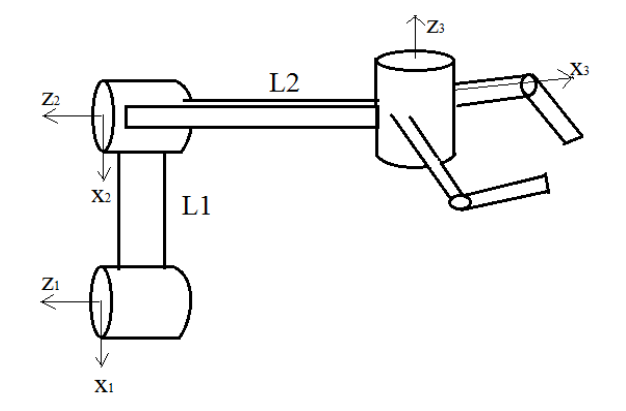
\includegraphics[width=6cm]{roboticarm.png}
\centering
\caption{The 3DOF robotic arm structure used, with coordinate frames}\label{net_img}
\end{figure}
The Robotic manipulator is described by Denavit Hartenberg (DH) Parameters as shown in Table 1. Where θirotational freedom of i-th joint, di  is translation freedom of ith joint, ai is  length of the joint which is the distance between yi and yi+1 axes. αiis the angle between xi and xi-1 axes.
\begin{table}[htdp]
\begin{center}
  \begin{tabular}{ | c | c |c|c|c|}
    \hline
    Link  & $\theta_i$ & $d_i$ & $a_i$ & $\alpha_i$ \\ \hline
    1     & $\theta_1$ & 0     & $L_1$ & 0\\ \hline 
    2     & $\theta_2$ & 0     & $L_2$ & 0 \\ \hline
    3     & $\theta_3$ & 0     & 0     & $90^o$ \\ \hline

  \end{tabular}
\end{center}
 \caption{D-H parameters of the designed robotic arm}\label{tab:a}
\end{table}

\begin{figure}[h]
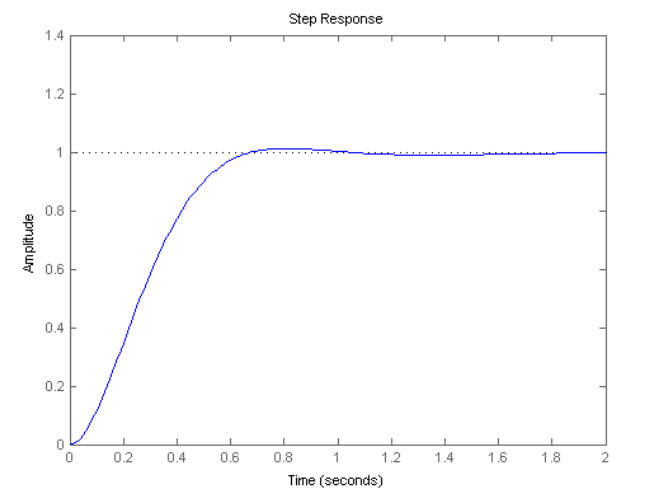
\includegraphics[width=6cm]{pidresponse.png}
\centering
\caption{Response of motor position with PID control}\label{net_img}
\end{figure}
\subsection{Object Detection}
Speeded Up Robust Features (SURF) [4] is a local feature detector and descriptor that is used for object recognition, classification and registration. It is inspired by Surface Invariant Feature Transform (SIFT) [4] and is several times faster than that and more robust.\\
To detect interest points, SURF uses Hessian blob detector. Its feature description is based on sum of Haar wavelet response around the point interest. These descriptors are used to recognize and track the objects.\\
\begin{figure}[h]
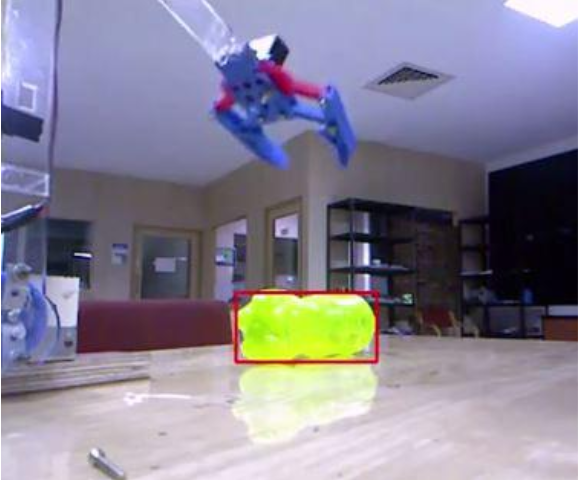
\includegraphics[width=6cm]{objectdetection.png}
\centering
\caption{Object detection}\label{net_img}
\end{figure}\\
Since the position of end-effector can be known using the forward kinematics and the position to be reached, final position is known by finding the desired object position through Kinect depth sensor, and then the final configuration, $C_g={\theta_{1g},\theta_{2g},\theta_{3g}}$ is calculated using inverse kinematics as shown in (2), (3).\\
\begin{equation} \label{eq:1}
cos\theta_2=\frac{x^2+y^2-l_1^2-l_2^2}{2l_1l_2}
\end{equation}\\
Using equation (1)\\
\begin{equation} \label{eq:2}
\theta_{2g}=atan2(+\sqrt{1-cos^2\theta_2},cos\theta_2)
\end{equation}\\

\begin{equation} \label{eq:3}
\theta_{1g}=atan2(y,x)-atan2(k_2,k_1)
\end{equation}\\
Where \\
$k_1=L_1+L2cos\theta_2$\\
$k_2=L_2+sin\theta_2$\\

Two Configurations are obtained which correspond to the elbow up and elbow down configurations of joint 2.\\
The torques $\tau$ of the motors is calculated by using (4).\\
\begin{equation} \label{eq:4}
\tau=J^TF
\end{equation}\\
Whereas J and F are shown in (5) and (6)
\begin{equation} \label{eq:5}
J=(-L_1S1+L_2S_12)L_1C1+L_2C12-L_2S12L_2C12
\end{equation}\\
considering the maximum limit
\begin{equation} \label{eq:6}
F=w_{end\ effector}+w_{load}+w_{motors\ and\ links}/2
\end{equation}\\

Where\\
J is the Jacobian\\
F is the force matix\\
w is the weight \\
$\tau$ is the torque\\
Position control of the DC Motor is done using PID control where the parameters are tuned manually to find the best response, since the system transfer function is unknown.\\
\begin{equation} \label{eq:7}
e= desired position- current position\\
\end{equation}
In discrete time steps\\
\begin{equation} \label{eq:8}
output\ Voltage=k_p*e_t+k_i\sum_{i=0}^{t}e_i+kd*(e_t-e_{t-1})
\end{equation}\\
\subsection{Mapping}
Real time mapping was done with the help of open source software, Real Time Appearance-Based Mapping (RTABMap). It is a novel RGB-D point cloud Simultaneous Localization and Mapping (SLAM) approach, which is based on a Bayesian loop Closure Detection [3]. This approach uses a bag of identifiers in the surrounding images to determine how likely a new image comes from a previous location or a new location. A loop closure is detected when the image is from the dataset of the previously collected images. RTABMap can be used directly with a hand-held Kinect or a stereo camera.
\subsection{wheel odometry}
The robot consisted of a differential drive mechanism for motion. Wheel encoders were used to calculate the rotational orientation of the wheels, to compute the velocity as well as the position information. The wheel odometry calculation consists of two parts.
\subsubsection{Linear Motion and Rotation Around Center of Axis}
\begin{figure}[h]
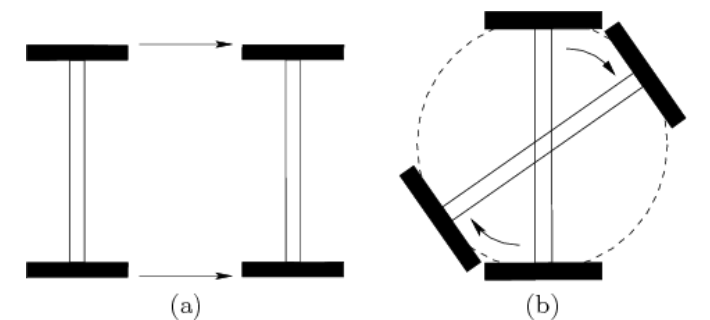
\includegraphics[width=6cm]{linearandrot.png}
\centering
\caption{(a)Linear motion of base, (b)Rotation about the central axis}\label{net_img}
\end{figure}
The linear velocity of the robot is given relation (8).
\begin{equation} \label{eq:9}
\vec{v}=\vec{R}\times \vec{\omega}
\end{equation}
Where\\
$\vec{v}$ is the linear velocity\\
$\vec{R}$ is the radius vector for the wheels\\
$\vec{\omega}$ is the angular velocity of the wheels\\
The rotational velocity of the robot is given by (8)\\
\begin{equation} \label{eq:10}
\omega_{bot}=\frac{v_r-v_l}{D}
\end{equation}
Where,\\
$\omega_{bot}$ is the angular velocity of the bot\\
D is the distance between the wheels\\
$v_r$ and $v_l$ are the velocities of the left and right wheels respectively\\

In this case $v_r$= - $v_l$.
\subsubsection{Rotation Around a Corner}

The displacement of the center of the robot can be given by (10).
\begin{equation} \label{eq:11}
S=\frac{r+b}{2}\theta
\end{equation}
Where,\\
S is the displacement\\
R is the distance of the corner form the nearest wheel\\
b is the distance between wheels\\
$\theta$  is the angle of rotation\\

\begin{figure}[h]
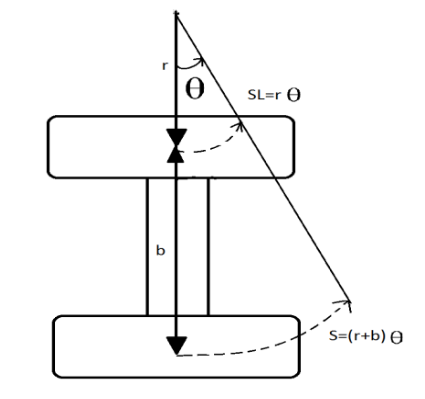
\includegraphics[width=6cm]{motionwithrotation.png}
\centering
\caption{The motion with rotation around a corner}\label{net_img}
\end{figure}

\subsubsection{Position Calculation}
The x and y axes velocities are given by (11) and (12).
\begin{equation} \label{eq:12}
\frac{dx}{dt}=\frac{v_r+v_l}{2}cos(\theta(t))
\end{equation}
\begin{equation} \label{eq:13}
\frac{dx}{dt}=\frac{v_r+v_l}{2}sin(\theta(t))
\end{equation}
Where,\\
m(t) is the velocity \\
$\theta(t)$ is the angular velocity of the center of base\\
The angular velocity is given by (13),\\
\begin{equation} \label{eq:14}
\frac{d\theta}{dt}=\frac{v_r-v_l}{2}
\end{equation}
The x and y positions and the orientation as a function of time are given by (14) and (15)\\
\begin{equation} \label{eq:15}
x(t)=x_o+\frac{b(v_r+v_l)}{2(v_r-v_l)}sin(\frac{(v_r-v_l)t}{b}+\theta_o)-sin(\theta_o)
\end{equation}

\begin{equation} \label{eq:16}
y(t)=y_o+\frac{b(v_r+v_l)}{2(v_r-v_l)}cos(\frac{(v_r-v_l)t}{b}+\theta_o)-cos(\theta_o)
\end{equation}

\begin{equation} \label{eq:17}
\theta(t)=\frac{v_r-v_l}{b}t+\theta_o
\end{equation}
Where,\\
$\theta_o$ is the initial orientation\\
$x_o$ is the initial x position\\
$y_o$ is the initial y position\\
\subsection{Sensor model and multi sensor bayesian inference}
The conditional Probability P(z $\mid$ x) [8] serves the role of a sensor model. In building a sensor model, the probability is constructed by fixing X = x, and finding P(z$\mid$ X=x) on z result. When this sensor model is used and observations are made Z = z is fixed and the likelihood function P(Z=z$\mid$x) on x is inferred. The multi sensor form of Bayes’ requires conditional independence as shown in (16). (17) States that posterior Probability [10] on x given by all observations $Z^n$ is simply proportional to the product of prior probability and individual likelihoods from each information source.
\\
\begin{equation} \label{eq:18}
P(x)=P(x)...P(z_n \mid x)
\end{equation}
\begin{equation} \label{eq:19}
P(x \mid Z^n)=CP(x)\prod_{i=1}^{n}P(z_i \mid x)
\end{equation}
Where\\
C is the normalization factor
\\
Here in our experiment, we are using $z_1$, which is visual Odometry from RTAB Map's [11] and $z_2$ is wheel Odometry. These are fused using the Bayesian filter [9].
\subsection{Localization}
Adaptive Monte Carlo Localization (AMCL) is a localization algorithm, which gives the position and orientation of the robot from the sensor data in the given environment. It uses particle filter to represent the distribution of likely states, with each particle representing a possible state which is hypothesis of where the robot is. Initially the algorithm starts with uniform random distribution of particles. Whenever the robot moves it shifts the particles to predict its new state after the movement. Whenever the robot senses something, the particles are resampled based on recursive Bayesian estimation to check how well the actual sensed data correlates with the predicted state.\\
Usually laser scans are used on ROS. But laser scanner are expensive. We used fake laser scan from the Kinect sensor. The 3D maps that are constructed with the RTABMap are made to 2D by projecting on to 2D Plane. This helps to know the obstacles of the robot in another 2D cross section of the 3D plane, which cannot be known with 2D laser scanner.
\section{Implementation}
All the algorithms were implemented over a laptop I 5 core, running Ubuntu 12.04. Robot Operating System (ROS Hydro) was used, with which the ROS Navigation Stack was used, for navigation and orientation control.
\\
The implementation can be divided into three parts

\subsection{Autonomous Navigation}
RTABMap was used to generate the 3D map form the point clouds obtained from Kinect. The visual odometry obtained from RTABMap was fused with the odometry data, computed from the rotary encoders in the wheels. This gave an accurate pose estimate of the robot, in the 3D environment.
\\
The 3D map was projected into a 2D occupancy grid, to mimic the data obtained form a LIDAR. This map was fed to the ROS Navigation Stack [ ], which was used to compute the most optimal path, to from destination to goal. The velocity commands sent from the NavStack were transformed into compatible commands and transferred to the motor controller over serial communication.
\subsection{Follow Me Mode}
The Skeleton markers package was used to track the human in front of the robot, in real time. It generates the 3D position for the skeletal joints. The coordinates of the center of the torso are given as input to the controller algorithm. The x coordinate is used to control the orientation of the robot, whereas the z coordinate is used to control the distance of the robot from the person being followed. The coordinates are fed to two PID controllers, to control the orientation and distance respectively. The set-points for the PID controllers are the center of the frame and a constant distance respectively. The following sequential logic is followed\\
-Detect the human skeleton and find the torso coordinates\\
-Use first PID controller to align the robot such that the person comes in the center of the frame, with a certain error margin\\
-Use the second PID controller, to move the robot towards or away from the person, depending on the distance set-point.\\
\subsection{Object Detectiona dnd Retreival}
 The object will be detected using SURF and a bounding box is made around the object. The center of the bounding box gives the (x, y) coordinates of the object, where the depth z of the object is obtained by finding the obstacle using one dimensional variation of IR along z, fixing x and y values. There will be sudden change in values of IR of Kinect sensor, at the object, which is an obstacle.
\begin{figure}[h]
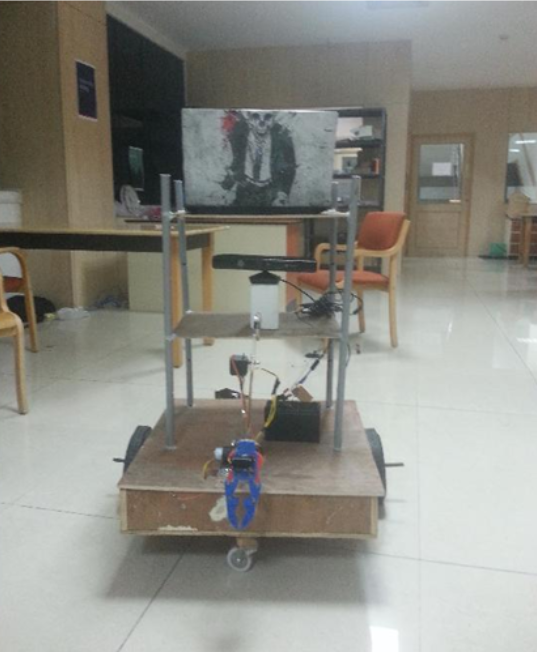
\includegraphics[width=6cm]{robotsetup.png}
\centering
\caption{The final setup of the robot}\label{net_img}
\end{figure}

\section{Conclusion}
The whole setup has been created in 600 USD. The efficiency is calculated by comparing  robot followed path with the the ideal path and is 95\%. 
\begin{figure}[h]
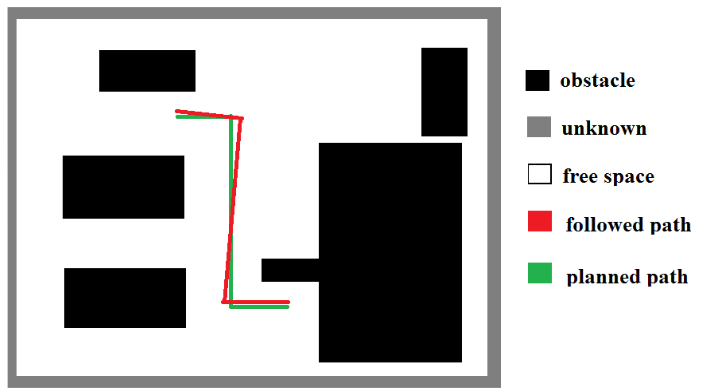
\includegraphics[width=8cm]{implementedresult.png}
\centering
\caption{Implemented result of path followed and planned}\label{net_img}
\end{figure}
\section*{Acknowledgment}
We would like to thank Texas Instruments, India for providing components to perform the experiment.


\begin{thebibliography}{1}
\bibitem{}
    Fox, Dieter, et al. \emph{Monte carlo localization: Efficient position estimation for mobile robots.} AAAI/IAAI 1999 (1999): 343-349. 
\bibitem{}
    Heitz, Fabrice, and Patrick Bouthemy. \emph{Motion estimation and segmentation using a global Bayesian approach.} Acoustics, Speech, and Signal Processing, 1990. ICASSP-90., 1990 International Conference on. IEEE, 1990. 
\bibitem{}
    Ho, Kin Leong, and Paul Newman. \emph{Detecting loop closure with scene sequences.} International Journal of Computer Vision 74.3 (2007): 261-286. 
\bibitem{}
   Juan, Luo, and Oubong Gwun. \emph{A comparison of sift, pca-sift and surf.}International Journal of Image Processing (IJIP) 3.4 (2009): 143-152.
\bibitem{}
    Cousins, Steve. \emph{Ros on the pr2 ros topics.} Robotics and Automation Magazine, IEEE 17.3 (2010): 23-25.
\bibitem{}
    Bohren, Jonathan, et al. \emph{Towards autonomous robotic butlers: Lessons learned with the pr2.} Robotics and Automation (ICRA), 2011 IEEE International Conference on. IEEE, 2011.
\bibitem{}
    Bischoff, Rainer, Ulrich Huggenberger, and Erwin Prassler. \emph{Kuka youbot-a mobile manipulator for research and education.} Robotics and Automation (ICRA), 2011 IEEE International Conference on. IEEE, 2011. 
\bibitem{}
   S. Thrun, W. Burgard, D. Fox:Probabilistic Robotics (MIT Press, Cambridge 2005)
\bibitem{}
   A. Elfes: Sonar-based real-world mapping and navigation,IEEETrans.Robot.Autom.3(3),249–265 (1987) 
\bibitem{}
    J.O. Berger: Statistical Decision Theory and Bayesian Analysis (Springer, Berlin, Heidelberg 1985).
\bibitem{}
    Labbé, Mathieu, and François Michaud. \emph{Memory management for real-time appearance-based loop closure detection.} Intelligent Robots and Systems (IROS), 2011 IEEE/RSJ International Conference on. IEEE, 2011.

\end{thebibliography}

\end{document}